% !TeX program = xelatex
\documentclass[a4paper,10pt]{article}

% ============================================================================
% សន្លឹកកិច្ចការសិស្សបំពេញចន្លោះ ស-ខ្មៅ និងប្លង់ក្ដារខៀន/ចម្លើយគ្រូ (គ្មាន LCD / គ្មានកន្ត្រៃ)
% មេរៀនទី៣ (២.៥)៖ ការប្រាក់សាមញ្ញ — ត្រូវគ្នា ១០០% នឹង LS_Plan_INT325.tex
% ============================================================================
\usepackage[a4paper, left=1.0cm, right=1.0cm, top=0.75cm, bottom=1.00cm, footskip=0.52cm]{geometry}
\usepackage{amsmath}
\usepackage{unicode-math}
\usepackage{fontspec}
\usepackage{array, colortbl}
\usepackage[table]{xcolor}
\usepackage{enumitem}
\usepackage{pifont}
\usepackage{fancyhdr}
\usepackage{lastpage}
\usepackage{tikz}
\usepackage[most]{tcolorbox}
\usetikzlibrary{calc, arrows.meta, decorations.pathreplacing, positioning, babel}

\makeatletter
\let\@expl@@@mark@update@singlecol@structures@@\relax
\makeatother

\providecommand{\NGSFindFonts}{%
  \IfFileExists{C:/Windows/Fonts/cambria.ttc}{%
    \def\NGSSysPath{C:/Windows/Fonts/}%
    \def\NGSUserPath{C:/Users/KIT/AppData/Local/Microsoft/Windows/Fonts/}%
  }{%
    \IfFileExists{./fonts/KhmerOSsiemreap.ttf}{\def\NGSSysPath{./fonts/}\def\NGSUserPath{./fonts/}}{%
    \IfFileExists{../fonts/KhmerOSsiemreap.ttf}{\def\NGSSysPath{../fonts/}\def\NGSUserPath{../fonts/}}{%
    \IfFileExists{../../fonts/KhmerOSsiemreap.ttf}{\def\NGSSysPath{../../fonts/}\def\NGSUserPath{../../fonts/}}{%
    \IfFileExists{../../../fonts/KhmerOSsiemreap.ttf}{\def\NGSSysPath{../../../fonts/}\def\NGSUserPath{../../../fonts/}}{%
    \IfFileExists{../../../../fonts/KhmerOSsiemreap.ttf}{\def\NGSSysPath{../../../../fonts/}\def\NGSUserPath{../../../../fonts/}}{%
    \IfFileExists{../../../../../fonts/KhmerOSsiemreap.ttf}{\def\NGSSysPath{../../../../../fonts/}\def\NGSUserPath{../../../../../fonts/}}{%
    \IfFileExists{../../../../../../fonts/KhmerOSsiemreap.ttf}{\def\NGSSysPath{../../../../../../fonts/}\def\NGSUserPath{../../../../../../fonts/}}{%
      \def\NGSSysPath{../../../../../../../fonts/}\def\NGSUserPath{../../../../../../../fonts/}%
    }}}}}}}%
  }%
}
\NGSFindFonts

\setmathfont[Path={\NGSSysPath}, FontIndex=1, Scale=1.02]{cambria.ttc}
\defaultfontfeatures{Ligatures=TeX}

\setmainfont[
  Path={\NGSUserPath}, Extension=.ttf, Script=Khmer,
  BoldFont={KhmerOSsiemreap}, BoldFeatures={FakeBold=1.8},
  ItalicFont={KhmerOSsiemreap}, ItalicFeatures={FakeSlant=0.25},
  BoldItalicFont={KhmerOSsiemreap}, BoldItalicFeatures={FakeBold=1.8, FakeSlant=0.25}
]{KhmerOSsiemreap}

\newfontfamily\muol[Path={\NGSUserPath}, Extension=.ttf, Script=Khmer]{KhmerOSmuollight}
\newfontfamily\TimesEn[Path={\NGSSysPath}, Extension=.ttf, BoldFont={timesbd}, ItalicFont={timesi}, BoldItalicFont={timesbi}]{times}
\newfontfamily\CalibriFont[Path={\NGSSysPath}, Extension=.ttf]{calibri}

\XeTeXlinebreaklocale "km"
\XeTeXlinebreakskip = 0pt plus 1pt minus 0.1pt

\definecolor{panelgray}{gray}{0.94}
\definecolor{headgray}{gray}{0.85}
\definecolor{midgray}{gray}{0.76}

\pagestyle{fancy}
\fancyhf{}
\renewcommand{\headrulewidth}{0pt}
\fancyfoot[L]{\fontsize{7.4pt}{9.5pt}\selectfont អនុវិទ្យាល័យព្រះក្រសាំង \en{|} គ្រូ៖ ហុក ប៊ុនថែន \en{|} មេរៀនទី៣ (២\en{.}៥) ការប្រាក់សាមញ្ញ \en{|} ថ្ងៃអង្គារ ទី២៤ ខែវិច្ឆិកា ឆ្នាំ២០២៦}
\fancyfoot[R]{\fontsize{7.8pt}{10pt}\selectfont ទំព័រ \en{\thepage\ / \pageref{LastPage}}}

\setlength{\parindent}{0pt}
\setlength{\parskip}{0pt}
\setlength{\tabcolsep}{4pt}

\newcommand{\en}[1]{{\TimesEn #1}}
\newcommand{\enbf}[1]{{\TimesEn\bfseries #1}}
\newcommand{\unit}[1]{\,\text{\en{#1}}}
\newcommand{\riel}{\,\text{៛}}
\newcommand{\usd}{\,\text{\en{\$}}}
\newcommand{\cnum}[1]{\mbox{\fontsize{10pt}{12pt}\selectfont\ding{\numexpr181+#1\relax}}}
\newcommand{\chkbox}{\tikz[baseline=-0.15ex]\draw[black, line width=0.85pt, fill=white] (0,0) rectangle (0.24cm,0.24cm);}
\newcommand{\ansbox}[1][1.55cm]{\,\tikz[baseline=-0.65ex]\draw[black, line width=0.65pt, fill=white] (0,0) rectangle (#1, 0.42cm);\,}
\newcommand{\dotline}[1][2.2cm]{\makebox[#1]{\dotfill}}

\newcommand{\pagebanner}[2]{%
  \begin{tcolorbox}[
    enhanced, sharp corners, colback=headgray, colframe=black,
    boxrule=1.05pt, boxsep=1pt, top=2.5pt, bottom=2.5pt, left=6pt, right=6pt,
    after skip=3.5pt
  ]
    {\muol\fontsize{9.0pt}{13.2pt}\selectfont #1}\hfill{\fontsize{8.0pt}{11.2pt}\selectfont\textbf{#2}}
  \end{tcolorbox}%
}

\newcommand{\secstrip}[2]{%
  \vspace{3pt}%
  \begin{tcolorbox}[
    enhanced, sharp corners, colback=panelgray, colframe=black,
    boxrule=0.8pt, boxsep=0.8pt, top=2pt, bottom=2pt, left=5pt, right=5pt,
    after skip=3pt
  ]
    {\muol\fontsize{8.5pt}{12.2pt}\selectfont #1}\hfill{\fontsize{7.8pt}{10.8pt}\selectfont\textit{#2}}
  \end{tcolorbox}%
}

\newcolumntype{L}[1]{>{\raggedright\arraybackslash}p{#1}}
\newcolumntype{C}[1]{>{\centering\arraybackslash}p{#1}}

\begin{document}
\fontsize{9.5pt}{14.5pt}\selectfont

% ============================================================================
% ទំព័រទី ១៖ សន្លឹកកិច្ចការសិស្ស (ផ្នែកមុខ៖ E1 -> E2 -> E3)
% ============================================================================
\pagebanner{សន្លឹកកិច្ចការសិស្ស \enbf{(}២\enbf{.}៥ ការប្រាក់សាមញ្ញ\enbf{)} \enbf{--} ផ្នែកមុខ}{ថ្នាក់ទី៨ \en{|} សៀវភៅគោល ទំ.៣៥--៣៦}

\begin{tcolorbox}[
  enhanced, sharp corners, colback=white, colframe=black,
  boxrule=0.8pt, boxsep=1.5pt, top=3.5pt, bottom=3.5pt, left=5pt, right=5pt,
  after skip=4pt
]
  \fontsize{9.0pt}{13.0pt}\selectfont
  \textbf{ឈ្មោះសិស្ស៖} \dotline[4.3cm] \quad
  \textbf{សមាជិកក្រុម៖} \dotline[4.3cm] \quad
  \textbf{ថ្នាក់ទី៖} ៨\dotline[0.9cm] \quad
  \textbf{ក្រុមទី៖} \dotline[1.0cm]
\end{tcolorbox}

% --- E1 Engage ---
\secstrip{ផ្នែកទី ១ \enbf{(E1 - Engage)} ៖ បេសកកម្មកុងត្រាខ្ចីប្រាក់កសិកម្មរយៈពេល ៦ ខែ}{រយៈពេល ៣ នាទី (គូស \ding{51} ក្នុង \chkbox)}

\begin{tcolorbox}[
  enhanced, sharp corners, colback=white, colframe=black,
  boxrule=0.8pt, boxsep=2pt, top=4pt, bottom=4pt, left=6pt, right=6pt
]
  សហគមន៍កសិកម្មឱ្យកសិករម្នាក់ខ្ចីប្រាក់ដើម $1\,000\,000\riel$ ដោយអត្រាការប្រាក់ \textbf{$12\%$ ក្នុង ១ ឆ្នាំ} សម្រាប់រយៈពេល \textbf{$6$ ខែ} ។\\[3pt]
  $\bullet$ \textbf{ការទស្សន៍ទាយរបស់ក្រុមអ្នក៖} \quad
  \chkbox\ \textbf{ស្មៀន សុខ៖} $720\,000\riel$ \qquad
  \chkbox\ \textbf{ស្មៀន តារា៖} $60\,000\riel$\\[3pt]
  $\bullet$ \textbf{ហេតុផលខ្លី៖} រយៈពេល $6$ ខែ ស្មើនឹងប៉ុន្មានឆ្នាំ? \dotline[3.0cm] ឆ្នាំ ។
\end{tcolorbox}

\vfill

% --- E2 Explore ---
\secstrip{ផ្នែកទី ២ \enbf{(E2 - Explore)} ៖ តារាងកើនការប្រាក់ថេរប្រចាំឆ្នាំ និងច្រកបំប្លែងខែទៅឆ្នាំ}{រយៈពេល ១១ នាទី}

\textbf{សកម្មភាព ១ (\en{E2-A} — ៦ នាទី)៖ ពូសំខ្ចីប្រាក់ធនាគារ $P = 2\,000\,000\riel$, អត្រា $R = 15\%$/ឆ្នាំ, រយៈពេល $T = 3$ ឆ្នាំ (ទំ.៣៦)}

\begin{tcolorbox}[
  enhanced, sharp corners, colback=white, colframe=black,
  boxrule=0.8pt, boxsep=2pt, top=4pt, bottom=4pt, left=6pt, right=6pt
]
  \centering
  {\renewcommand{\arraystretch}{1.35}
  \begin{tabular}{|C{2.4cm}|L{6.2cm}|L{4.2cm}|L{4.2cm}|}
    \hline
    \cellcolor{headgray}\textbf{រយៈពេល ($T$)} &
    \cellcolor{headgray}\textbf{ការគណនាការប្រាក់បង្គរ ($I$)} &
    \cellcolor{headgray}\textbf{ការប្រាក់សរុប ($I$)} &
    \cellcolor{headgray}\textbf{ប្រាក់សរុប ($A = P + I$)} \\
    \hline
    $1$ ឆ្នាំ & $2\,000\,000\times \dfrac{15}{100}\times 1$ & $300\,000\riel$ & $2\,300\,000\riel$ \\
    \hline
    $2$ ឆ្នាំ & $2\,000\,000\times \dfrac{15}{100}\times 2$ & \dotline[2.3cm] $\riel$ & \dotline[2.3cm] $\riel$ \\
    \hline
    $3$ ឆ្នាំ & $2\,000\,000\times \dfrac{15}{100}\times 3$ & \ansbox[2.2cm] $\riel$ & \ansbox[2.2cm] $\riel$ \\
    \hline
  \end{tabular}}
\end{tcolorbox}

\vspace{3pt}
\textbf{សកម្មភាព ២ (\en{E2-B} — ៥ នាទី)៖ ច្រកត្រួតពិនិត្យឯកតាពេលវេលា (ទំ.៣៥ — បើ $R$ ជា $\%$/ឆ្នាំ នោះ $T = \dfrac{\text{ចំនួនខែ}}{12}$ ឆ្នាំ)}

\begin{tcolorbox}[
  enhanced, sharp corners, colback=white, colframe=black,
  boxrule=0.8pt, boxsep=2pt, top=4pt, bottom=4pt, left=6pt, right=6pt
]
  បំប្លែងរយៈពេលខាងក្រោមទៅជាឯកតា\textbf{ឆ្នាំ} ឱ្យត្រូវគ្នានឹងអត្រាការប្រាក់ប្រចាំឆ្នាំ ($1\text{ ឆ្នាំ} = 12\text{ ខែ}$) ៖\\[3pt]
  ១) $6\text{ ខែ} = \dfrac{6}{12} =$ \dotline[1.5cm] ឆ្នាំ \qquad
  ២) $9\text{ ខែ} = \dfrac{9}{12} =$ \dotline[1.5cm] ឆ្នាំ \qquad
  ៣) $18\text{ ខែ} = \dfrac{18}{12} =$ \dotline[1.5cm] ឆ្នាំ
\end{tcolorbox}

\vfill

% --- E3 Explain ---
\secstrip{ផ្នែកទី ៣ \enbf{(E3 - Explain)} ៖ រូបមន្តការប្រាក់សាមញ្ញ រូបមន្តបញ្ច្រាស និងធនាគារហេតុផល \enbf{B\&W}}{រយៈពេល ៦ នាទី}

\begin{tcolorbox}[
  enhanced, sharp corners, colback=white, colframe=black,
  boxrule=0.85pt, boxsep=2pt, top=4pt, bottom=4pt, left=6pt, right=6pt
]
  $\bullet$ \textbf{រូបមន្តគោល (ទំ.៣៦)៖} តាង $P$ ប្រាក់ដើម, $R\%$ អត្រាក្នុង ១ ឆ្នាំ, $T$ រយៈពេល (ឆ្នាំ)៖ \quad
  $I = \dfrac{P \times R \times \dotline[0.8cm]}{100}$ \quad និង \quad $A = P + \dotline[0.8cm]$\\[5pt]
  $\bullet$ \textbf{រូបមន្តបញ្ច្រាស៖} \quad
  $R = \dfrac{100 \times I}{P \times T}$ \qquad ; \qquad
  $P = \dfrac{100 \times I}{\dotline[1.2cm]}$ \qquad ; \qquad
  $T = \dfrac{100 \times I}{\dotline[1.2cm]}$\\[4pt]
  \tikz\draw[black, dashed, line width=0.5pt] (0,0) -- (18.4cm,0);\\[3pt]
  \fontsize{8.8pt}{13.0pt}\selectfont
  \textbf{ធនាគារហេតុផល (\en{Warrant Bank})៖} \quad
  \cnum{1} \textbf{ប្រាក់ដើមថេរ៖} គិតលើ $P$ ដដែលរាល់ឆ្នាំ \quad
  \cnum{2} \textbf{ច្រកឯកតាឆ្នាំ៖} ខែត្រូវចែកនឹង $12$ ($T = \frac{m}{12}$)\\
  \cnum{3} \textbf{ញែកដាច់ $I$ និង $A$៖} ស្គាល់ប្រាក់សរុប $A$ ត្រូវដក $I = A - P$ សិន! \quad
  \cnum{4} \textbf{រូបមន្តបញ្ច្រាស៖} ជំនួសតម្លៃ $I$ សុទ្ធចូល $R = \frac{100I}{PT}$
\end{tcolorbox}

% ============================================================================
% ទំព័រទី ២៖ សន្លឹកកិច្ចការសិស្ស (ផ្នែកខាងខ្នង៖ E4 -> E5 -> កិច្ចការផ្ទះ)
% ============================================================================
\clearpage
\pagebanner{សន្លឹកកិច្ចការសិស្ស \enbf{(}២\enbf{.}៥ ការប្រាក់សាមញ្ញ\enbf{)} \enbf{--} ផ្នែកខាងខ្នង}{ថ្នាក់ទី៨ \en{|} សៀវភៅគោល ទំ.៣៦--៣៧, ៤២}

% --- E4 Elaborate ---
\secstrip{ផ្នែកទី ៤ \enbf{(E4 - Elaborate)} ៖ លំហាត់គំរូមីងថន តាមប្រអប់អថេរ \enbf{P--R--T--I--A} (ទំ.៣៦)}{រយៈពេល ១០ នាទី}

\begin{tcolorbox}[
  enhanced, sharp corners, colback=white, colframe=black,
  boxrule=0.8pt, boxsep=2pt, top=4pt, bottom=4pt, left=6pt, right=6pt
]
  \textbf{លំហាត់គំរូ (ទំ.៣៦)៖} មីងថនមានប្រាក់ដើម $15\,000\,000\riel$ ៖\\[3pt]
  $\bullet$ \textbf{ក. ផ្ញើនៅធនាគារអត្រា $6\%$ ក្នុង ១ ឆ្នាំ រយៈពេល $5$ ឆ្នាំ (ដកការប្រាក់រៀងរាល់ចុងឆ្នាំ — \cnum{1})៖}\\[2pt]
  \hspace*{0.3cm}ប្រអប់អថេរ៖ $P = 15\,000\,000\riel$, \quad $R =$ \dotline[1.0cm] $\%$, \quad $T =$ \dotline[1.0cm] ឆ្នាំ\\[3pt]
  \hspace*{0.3cm}$I = \dfrac{15\,000\,000 \times \dotline[0.8cm] \times \dotline[0.8cm]}{100} =$ \dotline[2.4cm] $\riel$ \quad $\implies$ \quad
  $A = P + I =$ \ansbox[2.6cm] $\riel$\\[4pt]
  $\bullet$ \textbf{ខ. ឱ្យមីងសានខ្ចី $15\,000\,000\riel$ រយៈពេល $2$ ឆ្នាំ ទទួលបានប្រាក់សរុប $A = 18\,000\,000\riel$ រកអត្រា $R$ (\cnum{3} + \cnum{4})៖}\\[2pt]
  \hspace*{0.3cm}-- \textbf{ជំហានទី១ (រកការប្រាក់សុទ្ធ \cnum{3})៖} $I = A - P = 18\,000\,000 - 15\,000\,000 =$ \dotline[2.4cm] $\riel$\\[3pt]
  \hspace*{0.3cm}-- \textbf{ជំហានទី២ (រកអត្រា \cnum{4})៖} $R = \dfrac{100 \times \dotline[2.0cm]}{15\,000\,000 \times 2} =$ \ansbox[1.6cm] $\%$ ក្នុង ១ ឆ្នាំ\\[3pt]
  \fontsize{8.8pt}{12.8pt}\selectfont
  \textbf{ឆ្លុះបញ្ចាំង (\en{EIA Looking-Back} \cnum{3})៖} ហេតុអ្វីមិនអាចជំនួស $18\,000\,000\riel$ ត្រង់ចូលខ្ទង់ $I$? ព្រោះ $18\,000\,000\riel$ គឺជាប្រាក់ \dotline[2.2cm] !
\end{tcolorbox}

\vfill

% --- E5 Evaluate ---
\secstrip{ផ្នែកទី ៥ \enbf{(E5 - Evaluate)} ៖ លំហាត់ប្រតិបត្តិ សំណួរវិនិច្ឆ័យ \enbf{A--D} និងសំបុត្រចេញ}{រយៈពេល ១០ នាទី}

\begin{minipage}[t]{0.52\textwidth}
  \begin{tcolorbox}[
    enhanced, sharp corners, colback=white, colframe=black,
    boxrule=0.8pt, boxsep=2pt, top=3.5pt, bottom=3.5pt, left=5pt, right=5pt,
    height=4.05cm
  ]
    \textbf{១) ប្រតិបត្តិ (ទំ.៣៦–៣៧ — ចឹកទ្រីខ្ចីប្រាក់ធនាគារ)៖}\\[2pt]
    ចឹកទ្រីខ្ចីប្រាក់ $P = 24\,000\,000\riel$ អត្រា $R = 16\%$/ឆ្នាំ រយៈពេល $T = 4$ ឆ្នាំ (បង់ការប្រាក់រៀងរាល់ឆ្នាំ) ៖\\[3pt]
    $\bullet$ \textbf{ក. ការប្រាក់សរុប៖} $I = \dfrac{24\,000\,000\times 16\times 4}{100} =$ \ansbox[1.75cm] $\riel$\\[4pt]
    $\bullet$ \textbf{ខ. ប្រាក់ត្រូវសងសរុប៖} $A = P + I =$ \ansbox[2.3cm] $\riel$
  \end{tcolorbox}
\end{minipage}\hfill
\begin{minipage}[t]{0.46\textwidth}
  \begin{tcolorbox}[
    enhanced, sharp corners, colback=white, colframe=black,
    boxrule=0.8pt, boxsep=2pt, top=3.5pt, bottom=3.5pt, left=5pt, right=5pt,
    height=4.05cm
  ]
    \textbf{២) បិទបេសកកម្ម \en{E1} និងលំហាត់រហ័ស៖}\\[2pt]
    $\bullet$ \textbf{បិទ \en{E1}៖} $P = 1\,000\,000\riel, R = 12\%, T = \frac{6}{12} = 0.5$ ឆ្នាំ៖\\[2pt]
    \hspace*{0.2cm}$I = \dfrac{1\,000\,000\times 12\times 0.5}{100} =$ \ansbox[1.9cm] $\riel$\\[4pt]
    $\bullet$ \textbf{លំហាត់រហ័ស៖} ផ្ញើ $3\,000\,000\riel$ បានការប្រាក់ $270\,000\riel$ ក្នុង $1$ ឆ្នាំ $\implies R =$ \dotline[1.4cm] $\%$
  \end{tcolorbox}
\end{minipage}

\vspace{4pt}

\begin{tcolorbox}[
  enhanced, sharp corners, colback=white, colframe=black,
  boxrule=0.8pt, boxsep=2pt, top=3.5pt, bottom=3.5pt, left=6pt, right=6pt
]
  \textbf{៣) សំណួរវិនិច្ឆ័យ \en{A--D} (ខ្ចីប្រាក់ $4\,000\,000\riel$ អត្រា $9\%$/ឆ្នាំ រយៈពេល $8$ ខែ រកការប្រាក់ $I$ — លើកម្រាមដៃ ១--៤)៖}\\[3pt]
  \textbf{\en{A.}} $2\,880\,000\riel$ \qquad\quad
  \textbf{\en{B.}} $240\,000\riel$ ($T = \frac{8}{12} = \frac{2}{3}$ ឆ្នាំ) \qquad\quad
  \textbf{\en{C.}} $360\,000\riel$ \qquad\quad
  \textbf{\en{D.}} $4\,240\,000\riel$\\[4pt]
  \tikz\draw[black, dashed, line width=0.5pt] (0,0) -- (18.4cm,0);\\[3pt]
  \textbf{៤) សំបុត្រចេញ ៦០ វិនាទី៖} (ក) $P = 500\,000\riel, R = 8\%/\text{ឆ្នាំ}, T = 3\text{ ឆ្នាំ} \implies I =$ \dotline[2.0cm] $\riel$ ។ \quad
  (ខ) ខ្ចី $2\,000\,000\riel$ រយៈពេល $1$ ឆ្នាំ សងសរុប $2\,300\,000\riel \implies$ ការប្រាក់ $I =$ \dotline[1.9cm] $\riel$ និងអត្រា $R =$ \dotline[1.2cm] $\%$ ។
\end{tcolorbox}

\vfill

% --- Homework ---
\begin{tcolorbox}[
  enhanced, sharp corners, colback=panelgray, colframe=black,
  boxrule=0.95pt, boxsep=2pt, top=4pt, bottom=4pt, left=6pt, right=6pt
]
  {\muol\fontsize{9.0pt}{13.0pt}\selectfont កិច្ចការផ្ទះ \enbf{(}សៀវភៅគោល ទំ.៤២ លេខ ១៦ និងលំហាត់អនុវត្តបំប្លែងខែ\enbf{)}}\\[3pt]
  \fontsize{8.9pt}{13.2pt}\selectfont
  $\bullet$ \textbf{\#16 (ទំ.៤២)៖} មីងដួនផ្ញើប្រាក់មួយចំនួននៅធនាគារ ។ បើធនាគារបញ្ចុះអត្រាការប្រាក់ប្រចាំឆ្នាំពី $15\%$ មកត្រឹម $13\%$ នោះការប្រាក់ប្រចាំឆ្នាំរបស់គាត់ថយចុះអស់ $200\,000\riel$ ។ ចូរគណនាប្រាក់ដើមដែលគាត់បានផ្ញើ ។\\[2pt]
  $\bullet$ \textbf{លំហាត់អនុវត្តបន្ថែម៖} ពូសុខាផ្ញើប្រាក់ $6\,000\,000\riel$ នៅគ្រឹះស្ថានមីក្រូហិរញ្ញវត្ថុដោយអត្រាការប្រាក់សាមញ្ញ $8\%$ ក្នុង ១ ឆ្នាំ រយៈពេល $9$ ខែ ។ ចូរគណនា (ក) ការប្រាក់សរុប $I$ និង (ខ) ប្រាក់សរុប $A$ ។ \textbf{អានមុន៖} ២.៦ ការប្រាក់សមាស (ទំ.៣៧--៣៨) ។
\end{tcolorbox}

% ============================================================================
% ទំព័រទី ៣៖ ទំព័រគ្រូបង្រៀន (គំរូប្លង់ក្ដារខៀន ៣ ផ្នែក + ចម្លើយផ្ទៀងផ្ទាត់រហ័ស)
% ============================================================================
\clearpage
\pagebanner{ទំព័រគ្រូបង្រៀន ៖ ប្លង់ក្ដារខៀន \enbf{(}គ្មាន \enbf{LCD)} និងចម្លើយផ្ទៀងផ្ទាត់រហ័ស}{២.៥ ការប្រាក់សាមញ្ញ (\en{INT325})}

\secstrip{១. គំរូប្លង់បែងចែកក្ដារខៀន ៣ ផ្នែក សម្រាប់ថ្នាក់រៀនគ្មាន \enbf{LCD}}{សម្រាប់គ្រូប្រើដីស/ហ្វឺត}

\begin{center}
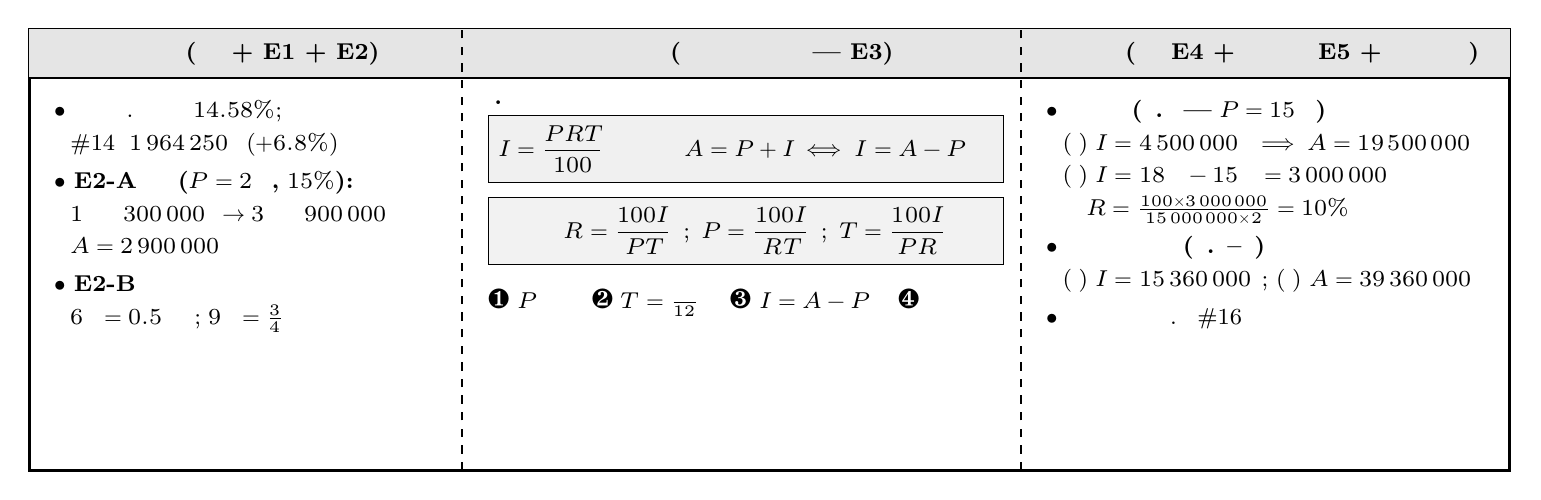
\begin{tikzpicture}[x=1cm, y=1cm, every node/.style={font=\fontsize{8.3pt}{11.8pt}\selectfont, text=black}]
  \draw[black, line width=1.1pt] (0,0) rectangle (18.8,5.60);
  \fill[gray!20] (0,4.98) rectangle (18.8,5.60);
  \draw[black, line width=0.7pt] (0,4.98) -- (18.8,4.98);
  \draw[black, dashed, line width=0.7pt] (5.5,0) -- (5.5,5.60);
  \draw[black, dashed, line width=0.7pt] (12.6,0) -- (12.6,5.60);

  \node at (2.75,5.29) {\textbf{ផ្នែកឆ្វេង (កំណែ + \en{E1} + \en{E2})}};
  \node at (9.05,5.29) {\textbf{ផ្នែកកណ្ដាល (ខ្លឹមសារគោលរក្សាទុក — \en{E3})}};
  \node at (15.70,5.29) {\textbf{ផ្នែកស្ដាំ (គំរូ \en{E4} + ប្រតិបត្តិ \en{E5} + កិច្ចការផ្ទះ)}};

  % Left
  \node[anchor=north west, text width=5.1cm] at (0.20,4.82) {%
    $\bullet$ \textbf{កំណែ៖} ទំ.៣៤ ចំណេញ $14.58\%$;\\
    \hspace*{0.2cm}\#14ខ $1\,964\,250\riel$ ($+6.8\%$)\\[2pt]
    $\bullet$ \textbf{\en{E2-A} ពូសំ ($P=2$លាន, $15\%$):}\\
    \hspace*{0.2cm}$1$ឆ្នាំ $300\,000\riel \to 3$ឆ្នាំ $900\,000\riel$\\
    \hspace*{0.2cm}$A = 2\,900\,000\riel$\\[2pt]
    $\bullet$ \textbf{\en{E2-B} ច្រកឯកតាឆ្នាំ៖}\\
    \hspace*{0.2cm}$6$ខែ $= 0.5$ឆ្នាំ; $9$ខែ $= \frac{3}{4}$ឆ្នាំ
  };

  % Center
  \node[anchor=north west, text width=6.7cm] at (5.70,4.82) {%
    {\muol\fontsize{8.5pt}{12pt}\selectfont ២\enbf{.}៥ ការប្រាក់សាមញ្ញ}\\[3pt]
    \tikz\node[draw=black, fill=gray!12, inner sep=3.5pt, text width=6.3cm]{%
      $I = \dfrac{PRT}{100}$ \quad និង \quad $A = P + I \iff I = A - P$
    };\\[4pt]
    \tikz\node[draw=black, fill=gray!10, inner sep=3.5pt, text width=6.3cm]{%
      បញ្ច្រាស៖ $R = \dfrac{100I}{PT}$ \,;\, $P = \dfrac{100I}{RT}$ \,;\, $T = \dfrac{100I}{PR}$
    };\\[4pt]
    \cnum{1} $P$ ថេរ \quad \cnum{2} $T = \frac{\text{ខែ}}{12}$ \quad \cnum{3} $I = A - P$ \quad \cnum{4} បញ្ច្រាស
  };

  % Right
  \node[anchor=north west, text width=5.8cm] at (12.80,4.82) {%
    $\bullet$ \textbf{គំរូមីងថន (ទំ.៣៦ — $P = 15$លាន)៖}\\
    \hspace*{0.2cm}(ក) $I = 4\,500\,000\riel \implies A = 19\,500\,000\riel$\\
    \hspace*{0.2cm}(ខ) $I = 18\text{លាន} - 15\text{លាន} = 3\,000\,000\riel$\\
    \hspace*{0.5cm}$R = \frac{100\times 3\,000\,000}{15\,000\,000\times 2} = 10\%$\\[2pt]
    $\bullet$ \textbf{ប្រតិបត្តិចឹកទ្រី (ទំ.៣៦–៣៧)៖}\\
    \hspace*{0.2cm}(ក) $I = 15\,360\,000\riel$; (ខ) $A = 39\,360\,000\riel$\\[2pt]
    $\bullet$ \textbf{កិច្ចការផ្ទះ៖} ទំ.៤២ \#16 និងលំហាត់ ៩ ខែ
  };
\end{tikzpicture}
\end{center}

\vspace{4pt}
\secstrip{២. ចម្លើយផ្ទៀងផ្ទាត់រហ័សសម្រាប់សន្លឹកកិច្ចការសិស្ស \enbf{(}ទំព័រ ១ និង ទំព័រ ២\enbf{)}}{\en{Answer Key}}

\begin{tcolorbox}[
  enhanced, sharp corners, colback=white, colframe=black,
  boxrule=0.8pt, boxsep=2pt, top=4pt, bottom=4pt, left=6pt, right=6pt
]
  \fontsize{9.0pt}{13.6pt}\selectfont
  $\bullet$ \textbf{ផ្នែក \en{E1}៖} ស្មៀនតារាត្រឹមត្រូវ ($60\,000\riel$); $6\text{ ខែ} = 0.5\text{ ឆ្នាំ}$ ។\\[2pt]
  $\bullet$ \textbf{ផ្នែក \en{E2}៖} \textbf{សកម្មភាព ១៖} $2$ ឆ្នាំ $\to I = 600\,000\riel, A = 2\,600\,000\riel$; $3$ ឆ្នាំ $\to I = 900\,000\riel, A = 2\,900\,000\riel$ ។ \textbf{សកម្មភាព ២៖} ១) $0.5$ (ឬ $\frac{1}{2}$) ឆ្នាំ; ២) $0.75$ (ឬ $\frac{3}{4}$) ឆ្នាំ; ៣) $1.5$ (ឬ $\frac{3}{2}$) ឆ្នាំ ។\\[2pt]
  $\bullet$ \textbf{ផ្នែក \en{E4}៖} (ក) $R = 6\%, T = 5 \implies I = 4\,500\,000\riel, A = 19\,500\,000\riel$ (\textit{កត់ចំណាំកំហុសពុម្ពសៀវភៅទំ.៣៦ ដែលដាក់ $1\,950\,000$}); (ខ) $I = 3\,000\,000\riel \implies R = 10\%$ ($18\,000\,000\riel$ គឺជាប្រាក់សរុប $A$) ។\\[2pt]
  $\bullet$ \textbf{ផ្នែក \en{E5}៖} \textbf{១) ចឹកទ្រី៖} (ក) $I = 15\,360\,000\riel$, (ខ) $A = 39\,360\,000\riel$ ។ \textbf{២) បិទ \en{E1}៖} $60\,000\riel$; លំហាត់រហ័ស $R = 9\%$ ។ \textbf{៣) វិនិច្ឆ័យ \en{A--D}៖} \textbf{ជម្រើស \en{B}} ($240\,000\riel$) ។ \textbf{៤) សំបុត្រចេញ៖} (ក) $120\,000\riel$; (ខ) $I = 300\,000\riel, R = 15\%$ ។
\end{tcolorbox}

\vspace{4pt}
\secstrip{៣. ចម្លើយលម្អិតនៃកិច្ចការផ្ទះ \enbf{(}សម្រាប់ផ្ទៀងនៅដើមម៉ោងបន្ទាប់ ២\enbf{.}៦\enbf{)}}{សៀវភៅគោល ទំ.៤២}

\begin{tcolorbox}[
  enhanced, sharp corners, colback=white, colframe=black,
  boxrule=0.8pt, boxsep=2pt, top=4pt, bottom=4pt, left=6pt, right=6pt
]
  \fontsize{8.9pt}{13.5pt}\selectfont
  $\bullet$ \textbf{\#16 (ទំ.៤២ — មីងដួនផ្ញើប្រាក់ធនាគារ)៖} តាង $P$ ជាប្រាក់ដើម ។ ក្នុងរយៈពេល $T = 1$ ឆ្នាំ អត្រាការប្រាក់ថយចុះពី $15\%$ មក $13\%$ គឺថយអស់ $15\% - 13\% = 2\%$ នៃប្រាក់ដើម ។ ដោយការប្រាក់ថយចុះ $200\,000\riel$ គេបាន៖ $\dfrac{P \times 2 \times 1}{100} = 200\,000 \implies P = \dfrac{200\,000 \times 100}{2} = \mathbf{10\,000\,000\riel}$ ។\\[3pt]
  $\bullet$ \textbf{លំហាត់អនុវត្តបន្ថែម (ពូសុខាផ្ញើប្រាក់ $9$ ខែ)៖} $P = 6\,000\,000\riel, R = 8\%$/ឆ្នាំ, បំប្លែង $T = \dfrac{9}{12} = \dfrac{3}{4}$ ឆ្នាំ ។\\
  (ក) ការប្រាក់សរុប $I = \dfrac{6\,000\,000 \times 8 \times \frac{3}{4}}{100} = 60\,000 \times 6 = \mathbf{360\,000\riel}$ ។ \quad
  (ខ) ប្រាក់សរុប $A = 6\,000\,000 + 360\,000 = \mathbf{6\,360\,000\riel}$ ។
\end{tcolorbox}

\end{document}
